% Created 2024-06-05 Wed 13:21
% Intended LaTeX compiler: pdflatex
\documentclass[a4paper,12pt, rulers]{tests2}
\usepackage[utf8]{inputenc}
\usepackage[T1]{fontenc}
\usepackage{graphicx}
\usepackage{longtable}
\usepackage{wrapfig}
\usepackage{tkz-fct}
\usepackage{tkz-euclide}
\usepackage{tkz-tab}
\usepackage{rotating}
\usepackage[normalem]{ulem}
\usepackage{amsmath}
\usepackage{amssymb}
\usepackage{capt-of}
\usepackage{hyperref}
\usepackage{exam-conf}
\renewcommand{\arraystretch}{1.2}
% \testtype{Contrôle}
% \period{{1 -- 2} -- \Circled{3 -- 4} -- 5 -- 6 -- {7 -- 8}}
% \materiel{Calculatrice}
% \testsection{5TTy}
% \testdate{17 juin 2024}
% \testlastname{Layeux}
% \testfirstname{Emma}
\newcommand{\IR}{\mathbb{R}}
\newcommand{\IZ}{\mathbb{Z}}
\newcommand{\IQ}{\mathbb{Q}}

\newcommand{\IN}{\mathbb{N}}
\renewcommand{\emptyset}{\varnothing}
\newcommand{\dom}{\mathrm{dom}}
\newcommand{\im}{\mathrm{im}}
\newcommand{\jdot}[1]{ \makebox[#1]{\dotfill}}
\newcommand{\tog}{\stackrel[<]{}{\to}}
\newcommand{\tod}{\stackrel[>]{}{\to}}
\newcommand{\pinf}{+\infty}
\newcommand{\minf}{-\infty}
\newcommand{\pminf}{\pm\infty}
\newcommand{\mpinf}{\mp\infty}
\newcommand{\FI}{\textbf{F.I.}}
\newcommand{\abs}[1]{|#1|}
\newcommand{\rad}{\text{rad}}
%\author{Quentin Lambotte}
%\date{2024-06-05}
%\title{\\\medskip
%\large 5UAA4}
\hypersetup{
 pdfauthor={Quentin Lambotte},
 pdftitle={},
 pdfkeywords={},
 pdfsubject={notes de cours de l'uaa4, 5GTT, math 4p},
 pdfcreator={Emacs 29.3 (Org mode 9.6.15)},
 pdflang={French}}

\providecommand{\tightlist}{%
  \setlength{\itemsep}{0pt}\setlength{\parskip}{0pt}}

\usepackage{exam-conf}
\renewcommand{\arraystretch}{1.2}
\period{\Circled{1 -- 2} -- {3 -- 4} -- 5 -- 6 -- {7 -- 8}}
\materiel{Pas de calculatrice}
\testsection{5TTy}
\testdate{17 juin 2024}
\testlastname{Layeux}
\testfirstname{Emma}\makeatletter\@ifpackageloaded{caption}{}{\usepackage{caption}}\AtBeginDocument{%
\ifdefined\contentsname
  \renewcommand*\contentsname{Table des matières}
\else
  \newcommand\contentsname{Table des matières}
\fi
\ifdefined\listfigurename
  \renewcommand*\listfigurename{Liste des Figures}
\else
  \newcommand\listfigurename{Liste des Figures}
\fi
\ifdefined\listtablename
  \renewcommand*\listtablename{Liste des Tables}
\else
  \newcommand\listtablename{Liste des Tables}
\fi
\ifdefined\figurename
  \renewcommand*\figurename{Figure}
\else
  \newcommand\figurename{Figure}
\fi
\ifdefined\tablename
  \renewcommand*\tablename{Table}
\else
  \newcommand\tablename{Table}
\fi
}\@ifpackageloaded{float}{}{\usepackage{float}}
\floatstyle{ruled}
\@ifundefined{c@chapter}{\newfloat{codelisting}{h}{lop}}{\newfloat{codelisting}{h}{lop}[chapter]}
\floatname{codelisting}{Listing}\newcommand*\listoflistings{\listof{codelisting}{Liste des Listings}}\makeatother\makeatletter\makeatother\makeatletter\@ifpackageloaded{caption}{}{\usepackage{caption}}
\@ifpackageloaded{subcaption}{}{\usepackage{subcaption}}\makeatother
\begin{document}

\begin{center}


\Large \textbf{ UAA4--Dérivée: \(\ldots/50\rightarrow \ldots\%\)}
\end{center}

\begin{abstract}
\begin{itemize}
\item Indique le nom et le prénom de ton ou ta voisin.e:\dotfill
\item Commencez par indiquer votre \textbf{NOM} et votre \textbf{Prénom} sur \textbf{chaque} feuille.
\item Vous avez \textbf{100 minutes} pour répondre à ce test.
\item \textbf{Lisez attentivement} l'énoncé de chaque question.
\item L'utilisation d'une calculatrice \textbf{est autorisée} mais l'échange de
calculatrices est interdit.
\item Vous pouvez utiliser le verso de chaque page comme
feuille de brouillon.
\end{itemize}
\end{abstract}
\newpage
\begin{question}<5>
Voici le graphique d'une fonction. Entoure la bonne réponse.

\begin{center}
  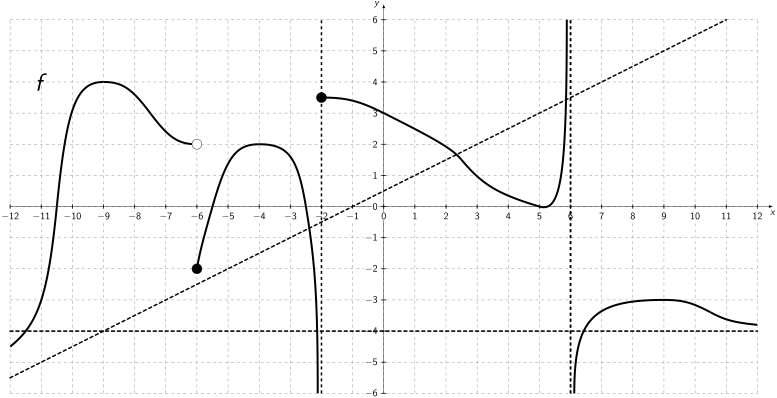
\includegraphics[width=0.7\linewidth]{fig/fig3.pdf}
\end{center}
\begin{center}
  \begin{tabular}{|l|llll|}
    \hline
    & \multicolumn{4}{l|}{Possibilités : entoure la bonne réponse}                                        \\ \hline
    $f'(-9)$                    & \multicolumn{1}{l|}{$<0$} & \multicolumn{1}{l|}{$=0$} & \multicolumn{1}{l|}{$>0$} & N’existe pas            \\ \hline
    $f'(-5)$                    & \multicolumn{1}{l|}{$<0$} & \multicolumn{1}{l|}{$=0$} & \multicolumn{1}{l|}{$>0$} & N’existe pas            \\ \hline
    $f'(0)$                     & \multicolumn{1}{l|}{$<0$} & \multicolumn{1}{l|}{$=0$} & \multicolumn{1}{l|}{$>0$} & N’existe pas            \\ \hline
    sur $]-2;5[$, $f'(x)$ est    & \multicolumn{1}{l|}{$<0$} & \multicolumn{1}{l|}{$=0$} & \multicolumn{1}{l|}{$>0$} & Le signe de $f'$ varie  \\ \hline
    sur $]-6;-2[$, $f''(x)$ est & \multicolumn{1}{l|}{$<0$} & \multicolumn{1}{l|}{$=0$} & \multicolumn{1}{l|}{$>0$} & Le signe de $f''$ varie \\ \hline
  \end{tabular}
\end{center}

\end{question}

\begin{question}<5>Voici le graphique d'une fonction \(f\).

  \begin{minipage}[r]{0.4\linewidth}
    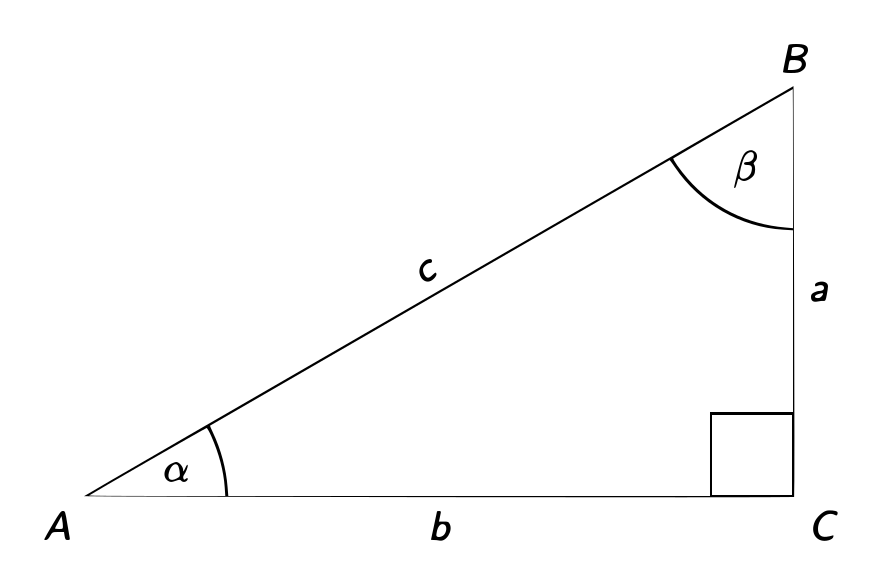
\includegraphics[width=\linewidth]{fig/fig4.pdf}
  \end{minipage}
  \begin{minipage}{0.59\linewidth}
    \begin{enumerate}
      \def\labelenumi{\arabic{enumi}.}  \tightlist
    \item Dresse le tableau de signes de \(f'\).

      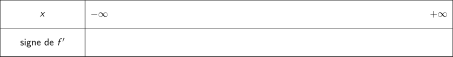
\includegraphics[width=\linewidth]{fig/tab3.pdf}

      \def\labelenumi{\arabic{enumi}.}  \setcounter{enumi}{1}
      \tightlist
    \item Dresse le tableau de signes de \(f''\).

      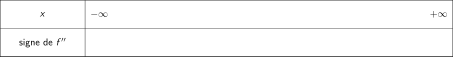
\includegraphics[width=\linewidth]{fig/tab4.pdf}

    \end{enumerate}
  \end{minipage}
\end{question}
\newpage
\begin{question}<14>
Calcule les dérivées suivantes.

\begin{enumerate}
\def\labelenumi{\arabic{enumi}.}
\tightlist
\item
  \(\left(\dfrac{x+1}{x-2}\right)'\) \vspace{5cm}
\item
  \(\left(\tan(x^2)+x^3\right)'\) \vspace{5cm}
\item
  \(\left(\cos(x^2+1)\right)'\) \vspace{5cm}
\item
  \(\left((x+2)(x+1)^4\right)'\) \vspace{5cm}
\item
  \(\left(\sin(2x)+x^3+1\right)'\) \vspace{5cm}
\item
  \(\left(\dfrac{1}{(x+1)^2}\right)'\) \vspace{5cm}
\item
  \(\left(\sqrt{x^2+x}\right)'\) \vspace{5cm}
\end{enumerate}

\end{question}

\newpage{}

\begin{question}<13>
Soit \(f(x)=x^3-3x^2-9x\).

\begin{enumerate}
\def\labelenumi{\arabic{enumi}.}
\item
  Calcule \(f'\) et \(f''\). Calcule ensuite les racines de ces deux
  fonctions.\vspace{5cm}
\item
  Construis le tableau de variations de \(f\)
\end{enumerate}

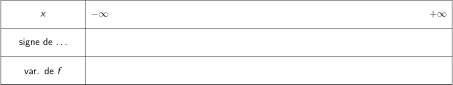
\includegraphics{fig/tab1.pdf}

\begin{enumerate}
\def\labelenumi{\arabic{enumi}.}
\setcounter{enumi}{2}
\item
  Donne les coordonnées des éventuels minimums et maximums.\vspace{3cm}
\item
  Construis le tableau de concavité de \(f\) .
\end{enumerate}

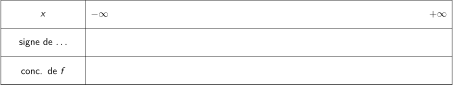
\includegraphics{fig/tab2.pdf}

\begin{enumerate}
\def\labelenumi{\arabic{enumi}.}
\setcounter{enumi}{4}
\tightlist
\item
  Donne les coordonnées des éventuels points d'inflexion.
\end{enumerate}

\end{question}

\newpage

\begin{question}<5> Détermine l'équation de la tangente au graphe de
\(f(x)=x^4+2x\) au point d'abscisse \(x=-1\). Donne tous les détails de
ton raisonnement.\end{question}
\vspace{5cm}
\begin{question}<8>
Une balle est lancée verticalement avec une vitesse initiale de 64m/s.
Le nombre de mètres au-dessus du sol après \(t\) secondes est donné par
la fonction suivante : \[
f(t)=-16t^2+64t+2
\]

\begin{enumerate}
\def\labelenumi{\arabic{enumi}.}
\tightlist
\item
  Sur quels intervalles \(f(t)\) est-elle croissante?
\item
  Quand est-ce que la hauteur est maximale? À quel moment la hauteur
  est-elle maximale?
\end{enumerate}

\end{question}
\end{document}
